%%%%%%%%%%%%%%%%%%%%%%%%%%%%%%%%%%%%%%%%%%%%%%%%%%%%%%%%%%%%%%%%%%%
% Method
% Team:
% Wolverine
% Members: 
% Eric Lee, Jacky Wu, Karthick Mani, 
% Eric Chang, Dexter Chen, Peter Chen
% Relative files:
% Method_Wolverine.tex, Library.bib, WolverineChart.png
% Note:    
% Do not compile this file compile Main.tex to get the pdf file instead.
%%%%%%%%%%%%%%%%%%%%%%%%%%%%%%%%%%%%%%%%%%%%%%%%%%%%%%%%%%%%%%%%%%%
	
\subsection{Built a database containing ten thousand articles}
%\textit{\footnotesize Author:Dexter Chen, Eric Chang, Eric Lee, Jacky Wu, Karthick Mani, Kenvin Lo, Yu-cheng Chen.}\\

The most important thing on this subject is to build a database which contains 10,000 articles. To reach that target, this study will go to discuss the advantages and disadvantages between different databases and will decide the most suitable one to be database of this study. At a meantime, this study will focus on how to use web crawlers to download articles automatically, which will contain in the database of this study.  

%Aim of this article is to give a brief idea of a database which is about to develop for the purpose of downloading the articles from open access databases using web crawler or web robot. And setting up a system that can allow the users to access the data in our database. we like to separate the article into 6 subsection based on their features, fallowed by then suggestions based on each feature. 


\subsubsection{Database Management Systems}

The relational database model was proposed by Edgar Codd in 1970, but because of the technological requirements it was not universal at that time. It was until 1980s that the first commercial relational database management systems began to appear.

A database management system (DBMS) is a computer software application that interacts with the user, other applications, and the database itself to capture and analyze data. Well-known DBMSs include MySQL, PostgreSQL, Microsoft SQL Server, Oracle, Sybase and IBM DB2. And they can support different kinds of databases.

%%%%%%%%%%%%%%%%% these are duplicated to the information following
%For building up such a database. We need a database management system (DBMS), a computer application that interacts with the user and other applications, captures and analyze data itself. Well-known DBMSs include MySQL, PostgreSQL, Microsoft SQL Server, Oracle, Sybase and IBM DB2. All of them can support different kinds of databases. This study includes numerous application and usage of such database as follows.
%MySQL is the second rank relational database management system (RDBMS) which is open-source. LAMP is an archetypal model of web service solution stacks, and its central component is MySQL. Web-based applications such as TYPO3 and MODx often use MySQL. MySQL is also applied in some famous website like Google, Facebook, and YouTube. It is able to be developed by the visual database design tool, MySQL Workbench.
%Same as Relational database, object-oriented database management systems has developed since the 1970s. Db4o which was launched in 2004 represents an object-oriented database model. It provides an easy interface to work with object-oriented programming languages and it also includes various object-oriented programming languages. For this reason, the programmer can work in one environment persistently.
%Finally, we'd like to introduce a DBMS, Neo4j. Neo4j is a graph database management system. It's one of the most popular GDBMS and ranks 20 in the popularity of DBMS. Unlike other databases, relationships take first priority in graph databases. Also, the model is simpler and expressive than those of relational databases, such as NOSQL databases. Neo4j is widely used by organizations and has 1,000,000+ downloads. Because Neo4j is easy to learn and use, it is more easier for beginners to get used to the structure of graph databases. This study also introduced three kinds of DBMS, and the following paragraph contains brief information about each kind of DBMS.

\begin{enumerate}
	\item\textbf{Object-oriented database}
	\setlength{\parindent}{1em}
	
	%An object-oriented database (OODBMS) is one of its kind, a database management system.\cite{WiKiauthor2013} The information in the database is represented as objects as used in object-oriented programming.
	
	An object database (also object-oriented database management system - OODBMS) is a database management system in which information is represented in the form of objects as used in object-oriented programming. Object databases are different from relational databases which are table-oriented.
	
	Because of tighter integration with the object-oriented language, the program is easier to maintain consistency with the same representation in both OODBMS and programming language.
	
	Although relational databases which are table-oriented might be similar to object-oriented databases, but they are actually different. The object-oriented database supports objects, classes, and inheritance in the database schema and query language.
	There are many advantages for OODBMS compared to the relational database management system (RDBMS) such as the performance, flexibility, and development cost.
	
	And OODBMS also have some disadvantages, the have mention 3 disadvantages for OODBMS. First, because the usage is forced to be similar to an object-oriented language. This makes maintaining and evolving is difficult. Second, the technique for store complex type of information takes additional computational resources. Third, the absence of a standard data model leads to design errors and inconsistencies.
	
	%And OODBMS also have some disadvantages, the \cite{Systems2010} have mention 3 disadvantages for OODBMS. First, because the usage is forced to be similar to an object-oriented language. This makes maintaining and evolving is difficult. Second, the technique for store complex type of information takes additional computational resources. Third, the absence of a standard data model leads to design errors and inconsistencies.
	
	\item\textbf{Relational database}
	\setlength{\parindent}{1em}
	
	A relational database is the most popular database used in the world. They can organize data into one or more tables of columns and rows, with a unique key identifying each row. Rows are also called records or tuples. Generally, each table represents one "entity type" (such as customer or product). The rows represent instances of that type of entity (such as "Lee" or "iPhone 6") and the columns representing values attributed to that instance (such as address or price).
	
	Considering the method of the organization of data, the relational database is much easier to understand and is flexible to manipulate the data. Besides SQL is easy in the relational database approach. For data organized in other structure, the query language either becomes complex or extremely limited in its capabilities. However, once the attributes of data become more and more, you'll need a large amount of tables to store your information. Therefore, the performance of relational database will decrease obviously.

	
	\item\textbf{Graph database}
	\setlength{\parindent}{1em}
	
	A graphical database uses graph structures for semantic queries with nodes, edges, and properties to represent and store data. Most graph databases are NoSQL in nature and store their data in a key-value store or document-oriented database. Graph databases are a powerful tool for graph-like queries, for example computing the shortest path between two nodes in the graph. Other graph-like queries can be performed over a graph database in a natural way.
	
	When Compare to relational databases, there are several advantages. A graph database is often faster for associative data set and map more directly to the structure of object-oriented applications. They can scale more naturally to large data sets as they do not typically require expensive join operations. As they depend less on a rigid schema, they are more suitable to manage ad hoc and changing data with an evolving schema.
	
	And graph database also comes with some disadvantages, the relational database is typically faster at performing the same operation on large numbers of data elements. AllegroGraph is one of the fine example for graph database. \\
	
	According to many database websites and discussion thread, there are several methods to store data in database. The two main directions are store inside the database and store out of the database. I will always be suggested not to store binary data in the database if the binary is large. That will cause significant performance decrease and additional storage space. And another way is to store binary data in the file system, and record the path in the database, that will not cause performance decrease when large binary data. But the binary data cannot automatically distribute with the database. Due to the PDF document will cost some performance issues even though PDF file is small in size and our system has no requirement to automatic distribute. We suggest sorting the PDF document in the file system.
	
\end{enumerate}

%\subsubsection{Database management system}
%The key feature which binds the relationship between user and administrator. Administrator's point of view, we like to give the best product to the end user. On the other hand, users strive to have convenient searching engine to find what they want at ease. For this purpose, I'm pressure to show two suggestions for enhancing the relationship between users and developer. First, setting up a word-ranking system. When user search for something with specific keyword, such as stem cell in medical area. In this moment, the word-ranking system will help the user by giving some suggested keywords. Of course, the word-ranking systems are developed based on users' searches and expert's suggestions to change the key words. This makes the system trust worthy.
 
%Secondly, building up a space in the database and allowing the user to change /edit the space based on their preference. The idea is referenced from well-known database, Wikipedia. It's so called "personalized searching".  By doing this, it would help user idealize their views on the system to what they want and suggest administrator the service which clients really want. It would lead to a win-win situation. 
	
	
\subsubsection{Web Crawler}
The web crawler is a program that can automatically browse through web pages, find out the information we assigned and store them. It has ability to process the data quickly and accurate to update a very large amount of data which are constantly being updated according to \cite{Liu2012}. It starts with a list of URL to visit, called the seeds. As crawler visits these URL, it identifies all the informations that we want, such as hyper links in the page and adds them to the list of URL to visit, called the crawl frontier. URL from the frontier is recursively visited according to a set of policies. If the crawler is performing archiving of websites, it copies and saves the information as it goes. The archives are usually stored in such a way they can be viewed, read and navigated as they were on the live web, but are preserved as 'snapshots' from \cite{Du2013}. We need to build up a web crawler to automatically visit a list of web page. Then find out which link in the page is valuable to download into our database.
	
	
%\subsubsection*{User account}
%One of the the main issue is how to create a user account that can connect between user and database. But the more important thing is to make sure database will not collapse by user who is not allowed to access to core part of database. 
 %To protect the database system security and privilege, this study introduces two methods for user account, principle of least privilege and role-based access control respectively. The principle of least privilege, also known as the principle of minimal privilege, means giving a user account only those those privileges which are essential to that user's work \cite{PrincipleLeastPrivilege}. The role-based access control is a policy neutral access control mechanism defined around privileges and roles. It can implement discretionary access control (DAC) or mandatory access control (MAC). The role-based access control is very easy to do user assignments as the components of this policy, such as role-permissions, etc. That is why it sometimes referred to as role-based security \cite{RoleBasedAccessControl}. The information and resources would not in danger due to these two methods will filter user depend on their authority and only allow the legitimate user to access. 
	
	
%\subsubsection*{User Interface}
%Understanding the types of visualizations people create by themselves for personal use. As part of this recent direction, we have studied a large collection of whiteboards in a research institution, where people make active use of combinations of words, diagrams and various types of visuals to help them further their thought processes. Our goal is to arrive at a better understanding of the nature of visuals that are created spontaneously during brainstorming, thinking, communicating, and general problem solving on whiteboards.\cite{Blascheck2016} We use the qualitative approaches of open coding, interviewing, and affinity diagramming to explore the use of recognizable and novel visuals, and the interplay between visualization and diagrammatic elements with words, numbers and labels. We discuss the potential implications of our findings on in- formation visualization design. Combining the advantage of visual thinking new standard of data processing, that visual nature of computers can challenge the first generation of hackers, An icon is an image, picture, or symbol representing a concept.\cite{Szpunar2010}
	
	
%\subsubsection*{Data Storage and Search Methods}
%The organization of data inside a database management system(DBMS) and retrieval methods is based on the database storage structure such as tables and indexes. There are several types of database storage structure such as XML, a textual data format. This advantage is self-describing and flexible in organizing data.\cite{ISI:000253400700005}Several considerations of data storage include right space allocation techniques, data compression techniques (if necessary), security and encryption and the access path to retrieve the data. Therefore, DBMS software will provide some method to optimize and minimum storage space of a database.
	
%\begin{figure*}[h]
%	\begin{center}
%		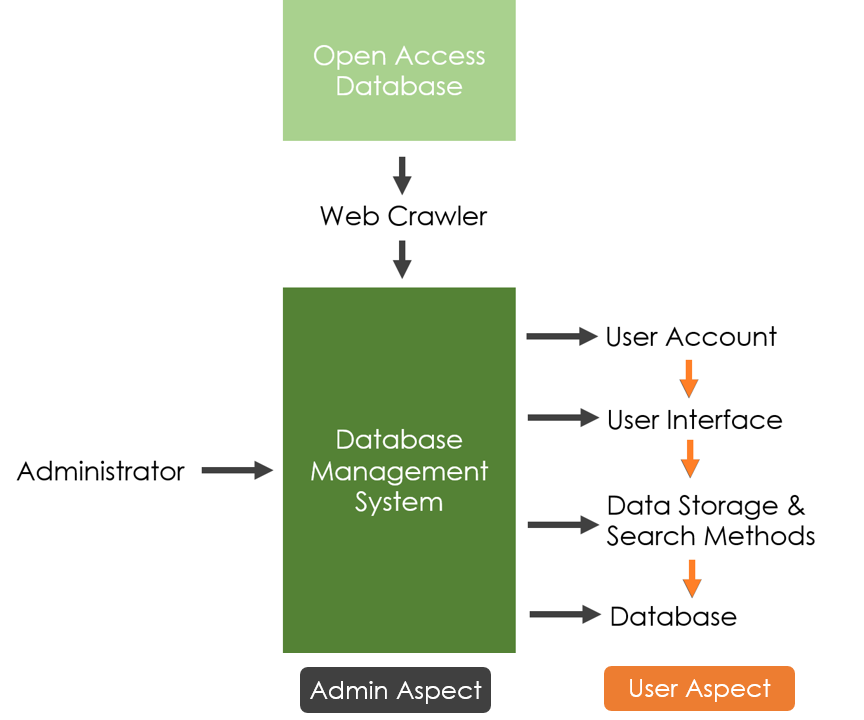
\includegraphics[scale=0.4]{WolverineChart}
%	\end{center}
%	\caption{Structure of our system}
%	\begin{center}
%		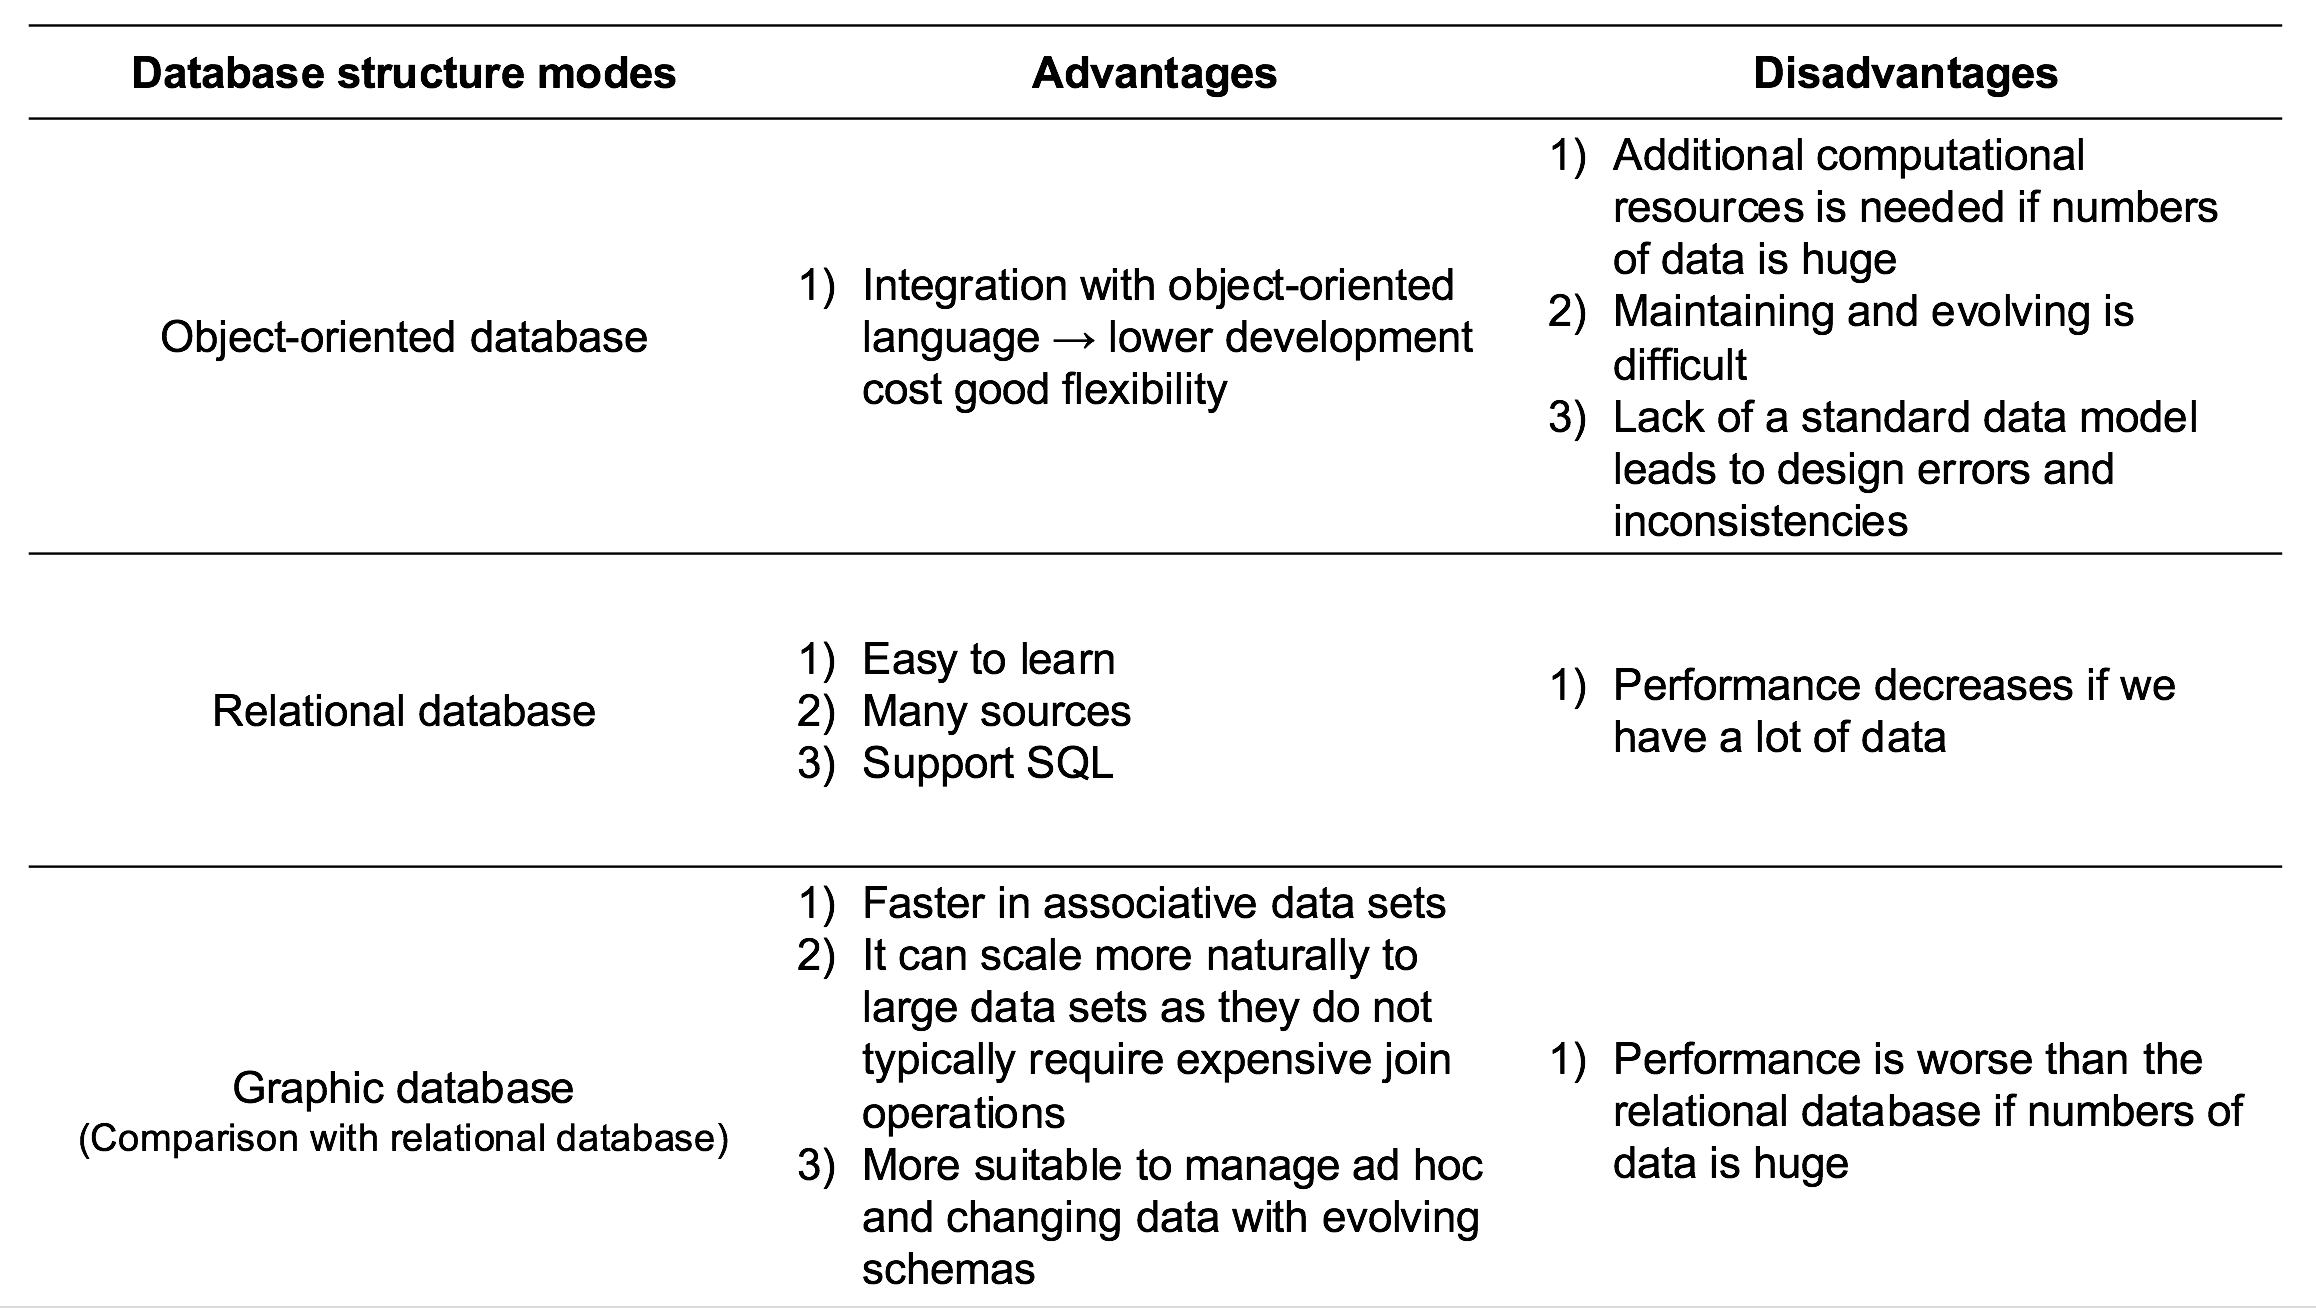
\includegraphics[scale=0.3]{WolverineChart2}
%	\end{center}
%	\caption{Database structure modes}
%\end{figure*}

\newpage % Ends the current page and causes all figures and tables to be printed
